% Chapter 3

\chapter{CHAPTER FOUR\\4.0 DATA ANALYSIS AND RESULTS} % Main chapter title
\section{Introduction}
In this chapter, we present the results of the data analysis. We also interpret and discuss the results. 

\subsection{Preliminary Results}
The study's data set includes time series of monthly EVI cases for the study area as well as various climatic factors like precipitation,Evaporation, the temperature (Tmin and Tmax), drought and relative humidity . After extracting all the data from  Google Earth Engine, there was a chance for correlation between observations because time series data points are gathered at close intervals. Instead of analyzing the imagery directly, we  summarize the data through descriptive statistics for the five variables under consideration are shown in Table 1. The numbers for EVI are 0.3945, 0.8672, and 0.7192, respectively, which are the minimum, maximum, and average levels. In terms of climatic factors, the minimum, maximum, and average values of Precipitation are 0.1203mm, 12.3576mm, and 3.9604mm, respectively. In contrast, the minimum, maximum, and average values of maximum temperature are 274.4C, 348.2C, and 309.3C, respectively. The original data's time series plots are shown in Figure 2, which clearly shows that both EVI and the climatic variables under consideration are seasonal. 
\subsection{Variable \& Parameter Definition}
Find in the tables (\textbf{4.2}) and (\textbf{4.3}) for the definition of variables and parameters respectively as used in this study. 
\begin{table}
	\label{Variable}
	\caption{Variable Definition.}
	\centering
	\begin{tabularx}{\textwidth}{ll}
		\hline\noalign{\smallskip}
		Variable & Definition \\ 
		\noalign{\smallskip}\hline\noalign{\smallskip}
		NDVI & Susceptible individuals \\  
		EVI & Exposed individuals \\ 
		Precipitation & Infected individuals \\ 
		Temperature & Recovered and Immunized individuals \\ 
		\hline\noalign{\smallskip}
	\end{tabularx}
\end{table}

 Figure 3's plot of the first difference in the data provides evidence of stationarity in both the climate Change and EVI variables.. This will shorten the analysis time while still providing an attractive and useful map. We will apply a smoothing strategy using an ARIMA function to fix the situation where some cells may not have  EVI for a particular month. Once NA values have been eliminated, the time series will be divided to eliminate seasonality before the normalized data is fitted using a linear model. We will go to classify our data on the map and map it after we have extracted the linear trend.
The 
To help machine learning classifiers work with time series data, we provide several new tools. We first contend that local features or patterns in time series can be found and combined to address challenges involving time-series categorization. Then, a method to discover patterns that are helpful for classification is suggested. We combine these patterns to create computable categorization rules. In order to mask low-quality pixels, we will first collect data from Google Earth Engine in order to choose  EVI values and Climate Change data.
\begin{table}[]
	\label{DataFrame}
	\caption{Data Collected from 2000-2022 on Google Earth Engine }
	\centering
	\begin{tabularx}{\textwidth}{@{}cllllll@{}}
		\toprule
		& \multicolumn{1}{c}{Vegetation Indices}   & \multicolumn{3}{c}{Climate Change}  \\ \midrule
		\multicolumn{1}{c}{Date} & \multicolumn{1}{c}{EVI} & \multicolumn{1}{c}{Precipitation} & \multicolumn{1}{c}{Evaporation} & \multicolumn{1}{c}{TempMin} & \multicolumn{1}{c}{TempMax} &\multicolumn{1}{c}{Drought}\\ \midrule
		
		
		2000-01-01&	-0.38280560&	1.0344619&	2.936857e-05&	217.1814&	315.8379&	-86.12496\\
		2000-02-01&	-0.08346374&	0.9917288&	2.634354e-05&	210.7751&	325.4743&	-168.35120\\
		2000-03-01&	0.46029681&	3.2132809&	2.927312e-05&	232.6620&	332.0389&	-220.69199\\
		2000-04-01&	0.68380747&	5.1810527&	4.515878e-05&	224.0424&	321.6810&	-190.38286\\
		2000-05-01&	0.25644143&	6.7150908&	4.758059e-05&	228.8765&	318.3983&	-210.67141\\
		2000-06-01&	-0.28410451&	8.2797964&	4.928518e-05&	222.4945&	295.6937&	-209.06835\\\bottomrule
		
	\end{tabularx}
\end{table}
\begin{table}[]
	\label{table:Summary Statistics}
	\caption{Summary statistics for Climate Date and Vegetation Loss In Ghana}
	\centering
	\begin{tabularx}{\textwidth}{|l*{3}{X|}*{3}{X|}}
		\toprule
		                   & Min.      & 1st Qu.& median & Mean & 3rd Qu & Max.  \\ \midrule
		EVI                &   0.3945  & 0.6423 & 0.7242 & 0.7168  & 0.8168&0.8672 \\
		Precipitation      &   0.1203  & 2.0311& 3.5497 &  3.9427 & 5.4892&12.3576 \\
		Evaporation & 1.682e-05 &3.595e-05&4.215e-05 &4.033e-05 & 4.560e-05&5.432e-05 \\
		TempMin            &   194.0 & 220.6  & 225.6  & 225.1 & 230.5 &242.7 \\
		TempMax            &   274.4 & 294.1 & 313.8& 309.0  &  322.2&348.2 \\ 
		Drought            &  -1354.42 & -339.45 & -228.47&-257.12 & -89.24&369.64 \\ \bottomrule
	\end{tabularx}
\end{table}
\subsection{Selection of Variables}
The purpose of this part is to examine how we got our answer and variables. First, we turned all categorical features into numerical attributes. Fortunaltely, some categroical features were already converted. Now, when we divided our variables into response and explanatory variables, some variables like dates and the unique policy number—were automatically discarded. Dates, policy number and other unrelevant variables which do not contribute to the project were removed, leaving us with these variables, PN, G, YOD, AOD, EL, MY, DUC, F, CAP, and NC

Again, we checked for the Pearson’s correlation between our target variable’s and the covariates’ which are presented in the below
\begin{figure}
	\centering
	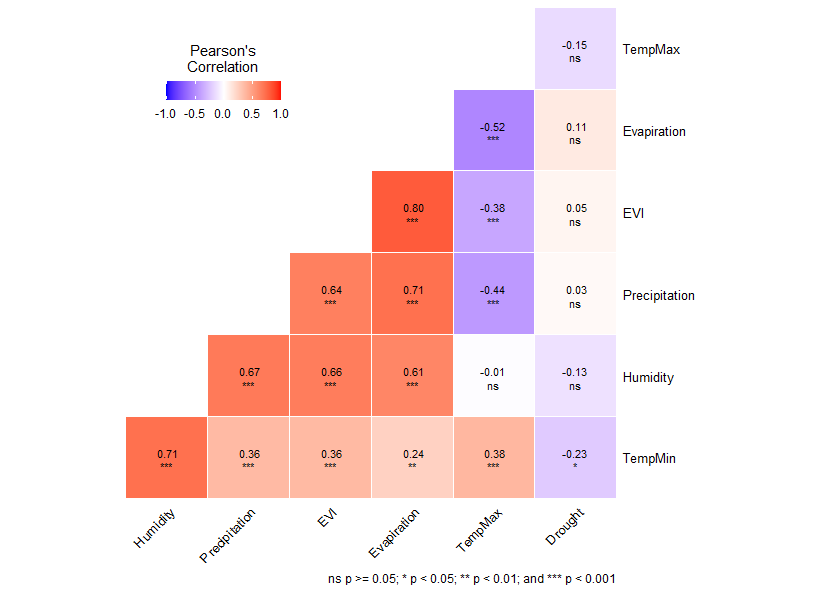
\includegraphics[width=0.9\linewidth]{images/Correlation}
	\caption{}
	\label{fig:Correlation}
\end{figure}

\subsection{Multicollinearity}
Although we have known about our study's target variable, EVI, from the outset, picking the covariates was a challenge. The following variables, with the exception of EVI, were intended to be used as covariates until it was discovered that multicollinearity among the covariates increases the sum of squared error..We employed the Variance Inflation Factor (VIF) to test for multi-collinearity, and the findings is shown in Table ~\ref{table:VIF},\\

\begin{center}
	\begin{table}
		
	\label{table:VIF}
	\caption{Best Variance Inflation Factor}
	\centering
	\begin{tabular}{|l|l|}
		\hline\hline
		Parameter	& Values \\
		\hline\hline
		Predictors	& 5 \\
		VIF	& 2.373 \\
		Condition number 	& 7.939\\
		Determinant 	& 0.2260766568 \\
		Selected 	& Drought, TempMin, Precipitation, TempMax, Evaporation \\
		Removed 	&  Humidity\\
		\hline
	\end{tabular}
  \end{table}
\end{center}
In order for our VIF score to fall between the ranges of 1 and 5, a piece of code was executed that automatically deleted variables with the highest VIF scores. The results of the chosen covariates are, This subsection statistically concluded that the variables Drought, TempMin, Precipitation, TempMax, and Evaporation will explain our target variable.


\subsection{Stationarity and Differencing}

Before building our models we first checked  if the series is stationary.We used the R program to do the ADF test, and we looked at many ADF test statistics to determine whether a unit root existed. This is essential to the VECM model and the VAR model in particular. That is, we needed to be determined that the time series is constant in mean and variance are constant and not dependent on time.Here, we look at a couple of methods for checking stationarity. If the time series is provided with seasonarity, a trend, or a change point in the mean or variance, then the influences need to be removed or accounted for. We use the Augmented Dickey–Fuller (ADF) t-statistic test to find if the series has a unit root (a series with a trend line will have a unit root and result in a large p-value).\parencite{dickey1979distribution}The test, shown in Tables ~\ref{(ADF) unit root test}, disproved the unit root hypothesis for all time series taken into account, suggesting that the relationships between the numerous variables investigated below are not fictitious.
\label{Chapter4} % For referencing the chapter elsewhere, use \ref{Chapter1} 
\begin{table}[]
	\label{table:(ADF) unit root test}
	\caption{Augmented Dickey Fuller (ADF) unit root test }
	\centering
	\addtolength{\tabcolsep}{4pt}
	\begin{tabularx}{\textwidth}{@{}cllllll@{}}
		\toprule
		& \multicolumn{3}{c}{EVI}   & \multicolumn{3}{c}{Precipitation}  \\ \midrule
		\multicolumn{1}{c}{} & \multicolumn{1}{c}{tau3} & \multicolumn{1}{c}{phi2} & \multicolumn{1}{c}{phi3} & \multicolumn{1}{c}{tau3} & \multicolumn{1}{c}{phi2} &\multicolumn{1}{c}{phi3}\\ \midrule
		
		Test-Statistics&-12.23373&49.89733&74.84565&-12.90546&55.54404&83.31586\\
		1pct&-3.98&6.15&8.34&-3.98&6.15&8.34\\
		5pct&-3.42&4.71&6.30&-3.42&4.71&6.30\\
		10pct&-3.13&4.05&5.36&-3.13&4.05&5.36\\ \bottomrule
		& \multicolumn{3}{c}{TempMin}   & \multicolumn{3}{c}{TempMax}  \\ \midrule
		\multicolumn{1}{c}{} & \multicolumn{1}{c}{tau3} & \multicolumn{1}{c}{phi2} & \multicolumn{1}{c}{phi3} & \multicolumn{1}{c}{tau3} & \multicolumn{1}{c}{phi2} &\multicolumn{1}{c}{phi3}\\ \midrule
		
		Test-Statistics&-9.292711&28.810535&43.191412&-9.219737&28.363876&42.545576\\
		1pct&-3.98&6.15&8.34&-3.98&6.15&8.34\\
		5pct&-3.42&4.71&6.30&-3.42&4.71&6.30\\
		10pct&-3.13&4.05&5.36&-3.13&4.05&5.36\\ \bottomrule
		
		& \multicolumn{3}{c}{Evaporation}   & \multicolumn{3}{c}{Drought}  \\ \midrule
		\multicolumn{1}{c}{} & \multicolumn{1}{c}{tau3} & \multicolumn{1}{c}{phi2} & \multicolumn{1}{c}{phi3} & \multicolumn{1}{c}{tau3} & \multicolumn{1}{c}{phi2} &\multicolumn{1}{c}{phi3}\\ \midrule
		
		Test-Statistics&-11.37318&43.16267&64.74007&-3.421750&3.915871&5.862217\\
		1pct&-3.98&6.15&8.34&-3.98&6.15&8.34\\
		5pct&-3.42&4.71&6.30&-3.42&4.71&6.30\\
		10pct&-3.13&4.05&5.36&-3.13&4.05&5.36\\
		
		\midrule\bottomrule
	\end{tabularx}
\end{table}
\section{VAR Estimation} With 12 lags for each variable in each equation, a VAR model of the monthly EVI and Climate Change variables was estimated. There are 4x12 unconstrained coefficients in each equation, plus one for a constant and one for a trend. Four tests were examine, the Final Prediction Error (FPE) test, the Hannan Quinne (HQ) test, the Information Criteria proposed by Akaike (AIC), and the Schwarz (SC) test were used to determine the appropriate number of lags. The results of all four tests suggested that up to 12 lagged monthly values would be sufficient. All the dynamics in the data are captured and employed in this analysis thanks to a lag duration of 12. (Table 3).

\begin{table}[]
	\label{table:Optimal lag}
	\caption{Optimal lag length selection}
	\centering
	\addtolength{\tabcolsep}{25pt}
	\begin{tabularx}{\textwidth}{@{}lllll@{}}
		\toprule
	 Lag  &	AIC(n)&	HQ(n)&	SC(n)&	FPE(n)\\\midrule
	1&	-8.242332&	-8.006335&	-7.655762&	0.0002633\\
	2&	-9.304816&	-8.866535&	-8.215470&	0.0000910\\
	3&	-9.743066&	-9.102502&	-8.150946&	0.0000588\\
	4&	-10.142686&	-9.299839&	-8.047791&	0.0000395\\
	5&	-10.286777&	-9.241647&	-7.689107&	0.0000343\\
	6&	-10.338471&	-9.091058&	-7.238027&	0.0000328\\
	7&	-10.345081&	-8.895385&	-6.741861&	0.0000328\\
	8&	-10.344697&	-8.692718&	-6.238702&	0.0000331\\
	9&	-10.310857&	-8.456595&	-5.702089&	0.0000347\\
	10&	-10.251454&	-8.194908&	-5.139910&	0.0000374\\
	11&	-10.250272&	-7.991444&	-4.635954&	0.0000382\\
	12&	-10.295256&	-7.834144&	-4.178163&	0.0000374\\
		 \bottomrule
	\end{tabularx}
\end{table}
\begin{figure}
	\centering
	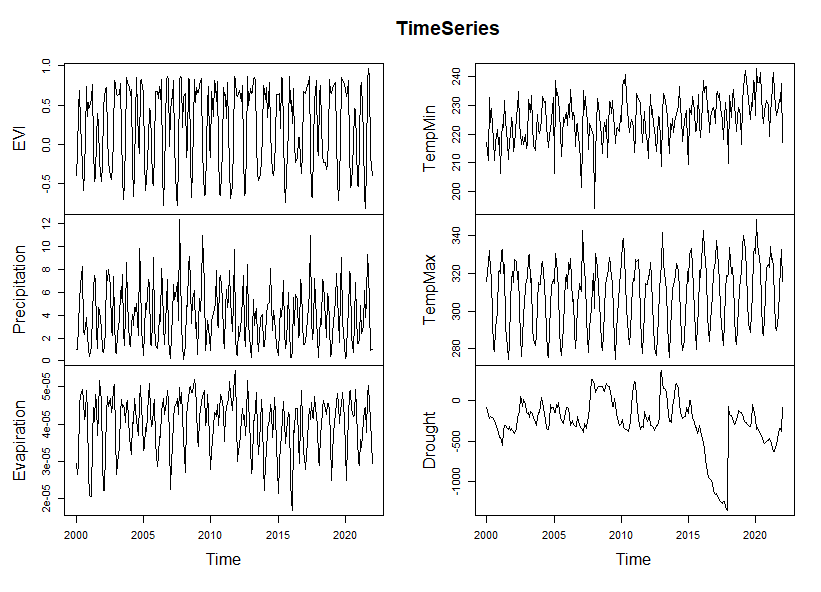
\includegraphics[width=0.9\linewidth]{images/TimeSeries}
	\caption{}
	\label{fig:TimeSeries}
\end{figure}
\begin{table}[]
	\label{table:Prediction}
	\caption{EVI forecast for the next 12 month.}
	\centering
	\addtolength{\tabcolsep}{25pt}
	\begin{tabularx}{\textwidth}{@{}lllll@{}}
		\toprule
   Month       & Forecast& Lower  &   Upper  &CI\\
   \bottomrule
 &-0.07548865& -0.65614302& 0.5051657& 0.5806544\\
 & 0.14803164& -0.56646127& 0.8625245& 0.7144929\\
 & 0.69105704& -0.04392727& 1.4260414& 0.7349843\\
 & 0.72499702& -0.05679272& 1.5067868& 0.7817897\\
 & 0.44066359& -0.41564183& 1.2969690& 0.8563054\\
 &-0.11537243& -0.98453117& 0.7537863& 0.8691587\\
 &-0.37165805& -1.24946226& 0.5061462& 0.8778042\\
 &-0.16672258& -1.05855108& 0.7251059& 0.8918285\\
 & 0.16015717& -0.73872579& 1.0590401& 0.8988830\\
 &  0.37177202& -0.53806829& 1.2816123& 0.9098403\\
 &  0.38160641& -0.53535068& 1.2985635& 0.9169571\\
 &  0.42144590& -0.49952777& 1.3424196& 0.9209737\\
		 \bottomrule
\end{tabularx}
\end{table}
\begin{table}[]
	\label{Optimal lag}
	\caption{Granger causality tests.}
	\centering
	\addtolength{\tabcolsep}{5pt}
	\begin{tabularx}{\textwidth}{@{}lllll@{}}
	\hline
	Cause variable &Null hypothesis& F-value& p-value& Decision\\
	\hline\hline
Precipitation	& does not Granger-cause &2.1563  & 0.01464  & Reject the null hypothesis  \\
	\hline
Evaporation	& does not Granger-cause & 1.5398 & 0.1112 &Fail to Reject the null hypothesis  \\
	\hline
TempMin	&  does not Granger-cause&3.0049  & 0.0006276 &Reject the null hypothesis  \\
	\hline
TempMax	& does not Granger-cause &2.7462  & 0.001685 &Reject the null hypothesis  \\
	\hline
Drought	& does not Granger-cause & 0.9235 & 0.5241 &Fail to Reject the null hypothesis \\
	\hline
\end{tabularx}
\end{table}
The dynamic interactions between EVI and the Climatic variables of the VAR (12) process were examined using impulse response analysis. Figure ~\ref{fig:impose} shows the orthogonal impulse response of EVI(Vegetation Condition) to the climate factors. The reaction of EVI exhibits a clear variation; the seventh month (July) has the largest negative effect of maximum temperature on EVI while we can see a rise in the Evaporation side and the third month has the lowest adverse effect (March). Additionally, the third month (March) is when relative humidity has the most positive impact on malaria, whereas the tenth month (October) is when rainfall has the greatest good impact (October).
\begin{figure}
	\centering
	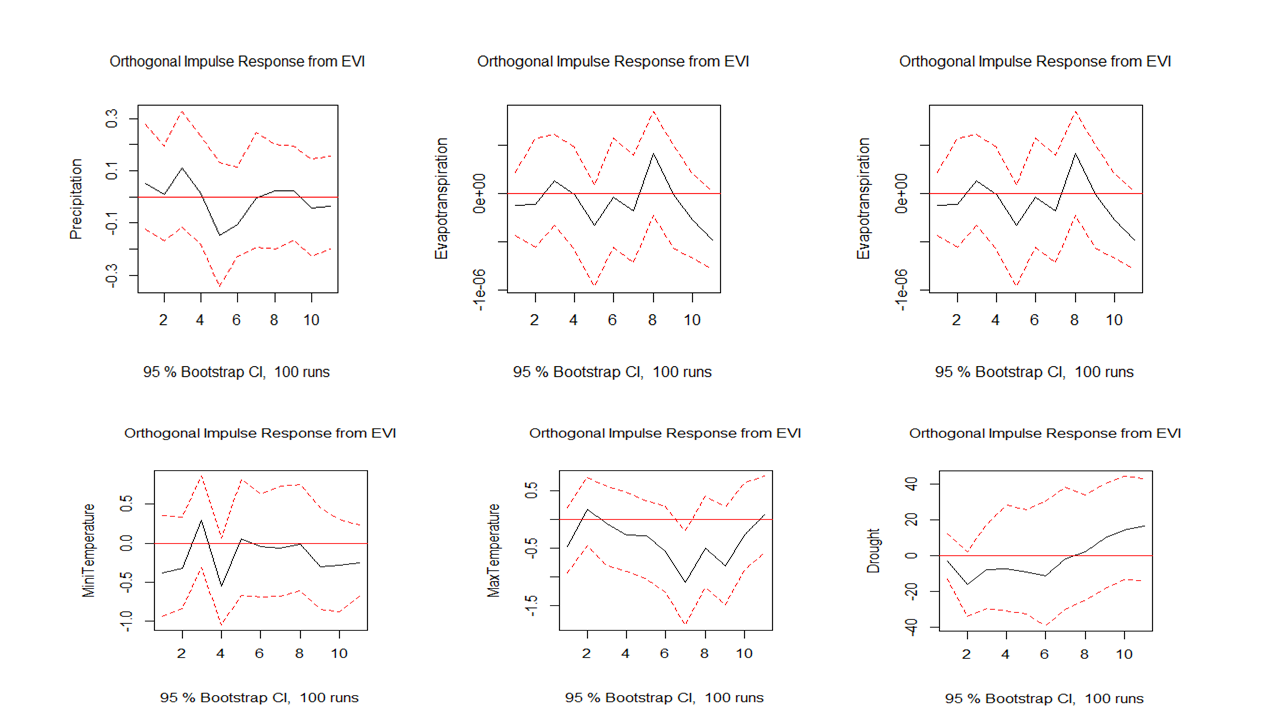
\includegraphics[width=1\linewidth]{images/impose}
	\caption{}
	\label{fig:impose}
\end{figure}
\subsection{ Decomposition of Variance}
In order to evaluate VAR models, many people use forecast error variance decomposition (FEVD). Figure ~\ref{fig:fevd} displays the results for the FEVD for malaria and the climate factors. The findings show that, on average, past values EVI(Vegetation Condition)  account for about 85.67\% of the variability in the trend of malaria, while past innovations in maximum temperature account for a sizable percentage (around 5.65\%) of the variability in the trend of EVI. Additionally, although earlier advances in Evaporation data have been able to account for around 3.10 percent of the variability in the trend of EVI, past innovations in relative Precipitation have only been able to account for 0.58 percent of that variability.
\begin{figure}
	\centering
	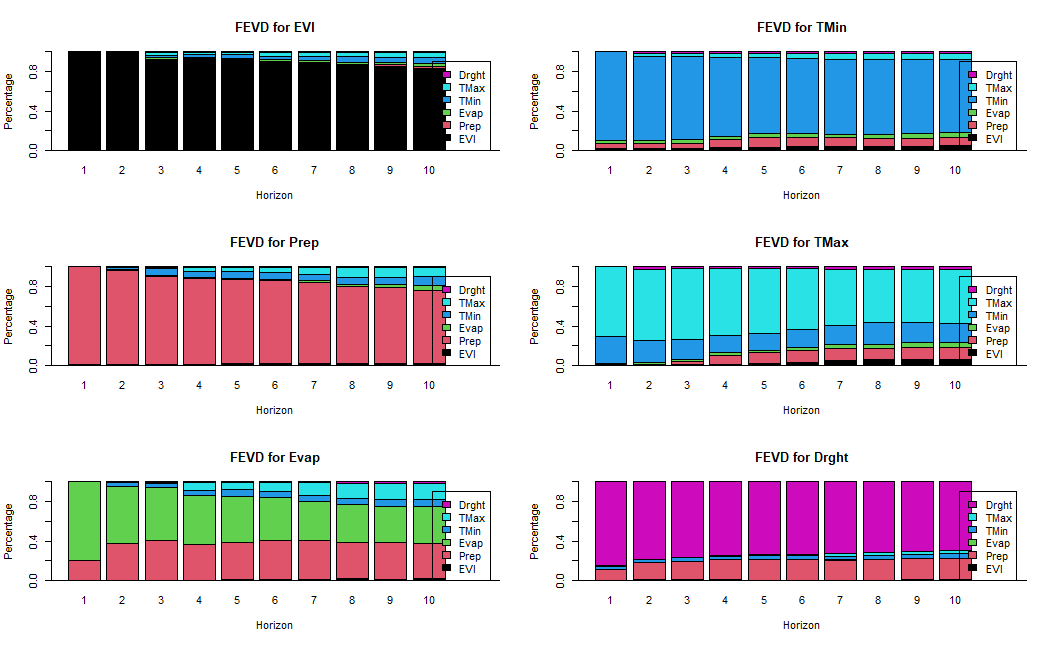
\includegraphics[width=0.9\linewidth]{images/fevd}
	\caption{}
	\label{fig:fevd}
\end{figure}
\subsection{Forecast for EVI} Future EVI  cases can be predicted using the created VAR (12) model as a predictive model. Figure  and Table  both revert the forecasts for the number of differed EVI during the first half of 2022 to the original level. These predictions

\subsection{Prediction accuracy} Regardless of whether the forecasting mistake is positive or negative, the mean absolute percentage error (MAPE) gives a general idea of the average size of forecasting error represented as a \% of the actual observed number . The fitted model's MAPE is calculated to be 12.95\% using (14) which suggests that its projections may be quite accurate .

The Granger and immediate causality tests reveal that only three climate factors have an impact on malaria. The impulse response analyses show that the ninth, third, and tenth months, respectively, had the strongest favorable effects of maximum temperature, relative humidity, and rainfall on malaria. With less than 20\% of the variability in the trend of EVI being explained by historical innovations in Climate Change, the decomposition of predicted variance shows varied degrees of EVI dependence on climatic variables. Policymakers can utilize the study's findings to assist them develop policies by understanding how climatic variability affects the incidence of EVI in the Study Area.

Area.